%\documentclass[../main/6103-LecturesNotes.tex]{subfiles}
%\begin{document}

\section{Exponentials}
We have seen functions of the form $f(x)=x^a$, where $a$ is a constant. What happens if we swap the $a$ and the $x$ and look at $f(x)=a^x$?

First, let's look at what $a^x$ means for all values of $x\in\mathbb{R}$.

\subsection{Indices}
when we wish to multiply a number by itself several times, we make use of index or power notation. We have notation for powers (for \(a\in\mathbb{R}\):
\begin{align*}
&a^2=a\cdot a\quad\\
&a^3=a\cdot a\cdot a\\
&a^x=\overbrace{a\cdot a \dots a\cdot a}^x \quad x\in\mathbb{N}\text{ and }x\not=0
\end{align*}

Here, $a$ is called the \textbf{base} and $x$ is called the \textbf{index} or \textbf{power}. We also know the following properties:
\begin{thing}{Properties of exponents}
For any $a\in\mathbb{R}$ and $x,y\in\mathbb{R}$
\begin{enumerate}
\item $a^{x+y}=a^x\cdot a^y$

\item $\left( a^x \right)^y=a^{xy}$

\item $a^x \cdot b^x = \left( ab \right)^x$
\end{enumerate}
\end{thing}

\begin{examples}
\begin{enumerate}
\item $2^5=2 \cdot 2 \cdot 2 \cdot 2 \cdot 2 =2^3 \cdot 2^2$.

\item $3^6=3^{2\times 3}=3 \cdot 3 \cdot 3 \cdot 3 \cdot 3 \cdot 3 = 3^2 \cdot 3^2 \cdot 3^2 = (3^2)^3$.

\item $2^3\cdot 3^3 = 2 \cdot 2 \cdot 2 \cdot 3 \cdot 3 \cdot 3=(2 \cdot 3)(2 \cdot 3)(2 \cdot 3)=(2 \cdot 3)^3$.
\end{enumerate}

\end{examples}

We can use the properties of exponents to justify the definitions of \(a^x\) when \(x\) is not a positive integer. Throughout this we will assume that \(a>0\).

\subsubsection{For \(x\in\mathbb{Z}\)}
For \(x=0\), we notice that:
\begin{align*}
a^2 &= a^{2+0}\\ &= a^2\cdot a^0
\end{align*}
This shows that:
\begin{in_a_box}
$$a^0=1$$
\end{in_a_box}

When \(x\) is a negative integer:
\begin{align*}
1 &= a^0\\ &= a^{x-x}\\ &= a^x\cdot a^{-x}
\end{align*}
Dividing by \(a^{x}\), we get:
\begin{in_a_box}
$$a^{-x}=\frac{1}{a^x}$$
\end{in_a_box}

\subsubsection{For \(x\in\mathbb{Q}\) (the set of all fractions)}

For \(x=\frac{1}{n}\), notice that:
\begin{align*}
\left(a^{\frac{1}{n}}\right)^n &= a^{\frac{1}{n}\cdot n}\\ &= a^1\\ &= a
\end{align*}

Taking the \(n\)th root gives:
\begin{in_a_box}
$$a^\frac{1}{n} = \sqrt[n]{a}$$
\end{in_a_box}

Similarly, we find that
\begin{in_a_box}
$$a^\frac{m}{n} = \left(\sqrt[n]{a}\right)^m$$
\end{in_a_box}

\subsubsection{For \(x\in\mathbb{R}\)}

If $x$ is an irrational number, then, for any small number \(\epsilon>0\) we can always find two rational numbers $c$ and $d$ which satisfy $x-\epsilon<c<x<d<x+\epsilon$.
$a^x$ is defined to be the limit of \(a^c\) (or \(a^d\)) as \(\epsilon\rightarrow0\).

Finally, an exponential function can be defined by
\begin{equation*}
f(x)=a^x,\quad x\in\mathbb{R},
\end{equation*}
where $a$ is a positive constant. The domain of $f$ is $\mathbb{R}$ and the range is $\mathbb{R}^+$. 

If \(a<1\), it is common to define \(b=\frac{1}{a}\). \(f\) can then be written as \(f(x)=b^{-x}\) with \(b>1\).

The graph of f is as follows:

\begin{figure}[H]
    \hspace{0.2cm}
    \subfigure[$y=a^x,\quad a>1$.]{\label{fig:exponent-graph1}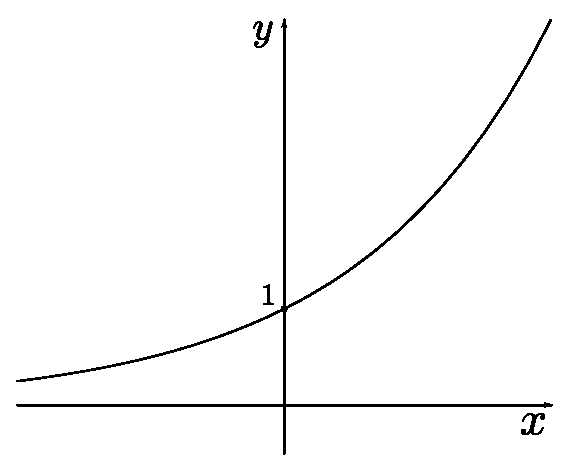
\includegraphics[scale=0.6]{img/exponent-graph1}}
    \hspace{2.0cm}
    \subfigure[$y=a^{-x},\quad a>1$.]{\label{fig:exponent-graph2}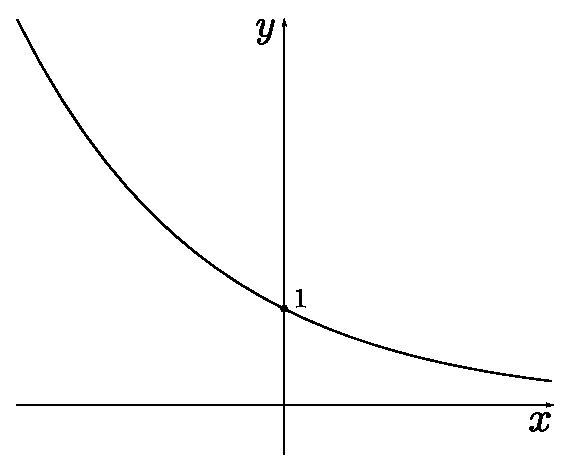
\includegraphics[scale=0.6]{img/exponent-graph2}} \\
    \centering
  \caption{Comparison of exponent graphs for different values of $a$.}
  \label{fig:exponent-graphs}
\end{figure}

There is also a special exponential function, $f=e^x$, we will investigate this further later in the course.


%\end{document}
